\chapter{Performance}
In this chapter we will explain the used metodology to evaluate the performance of the model. We will also show the results of the training and the evaluation of the model on the test set with proper examples for good and bad predictions.


\section{Training Results and Evaluation}
The model was trained for 50 epochs. We got the best results in the 32th epoch. The training loss and the validation mAP are shown in the following figure \ref{fig:loss}.


\begin{figure}[ht]
    \centering
    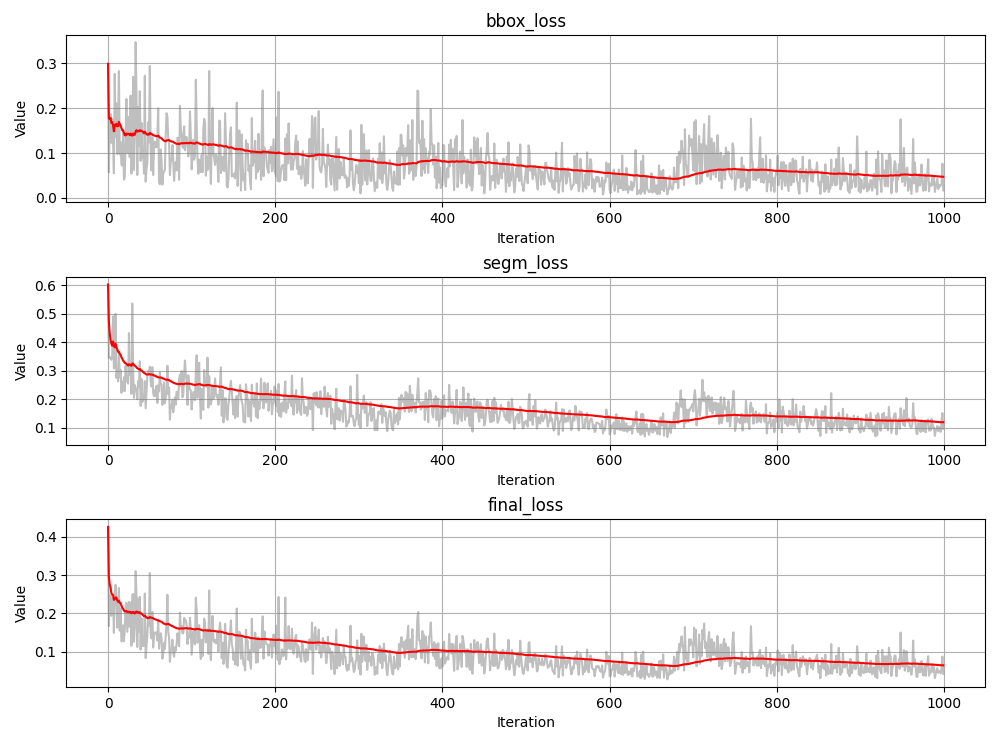
\includegraphics[width=0.9\textwidth]{Images/lossess.png}
    \caption{Training lossess}
    \label{fig:loss}

    \vspace{0.5cm}

    \centering
    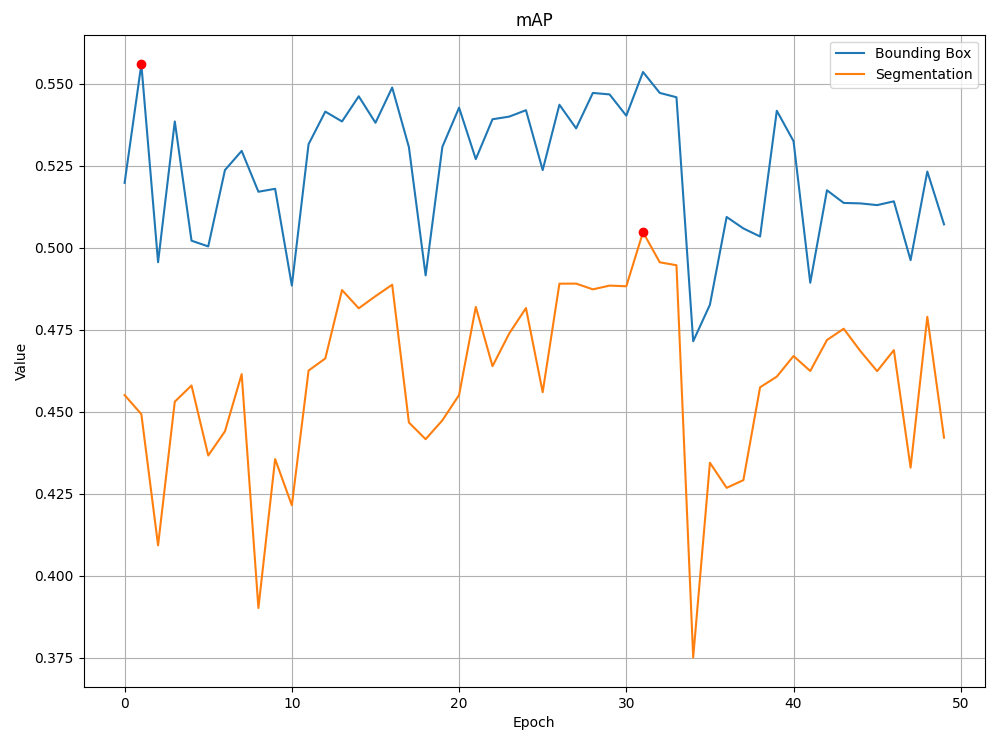
\includegraphics[width=0.9\textwidth]{Images/val_acc.png}
    \caption{Evaluation on the test set during training. Points are the best mAP values for the Bounding Box and the Segmentation Mask. The best model is at epoch 32.}
    \label{fig:evaluation}
\end{figure}

To evaluate the model we used the Mean Average Precision (mAP) metric for both the Bounding Box and the Segmentation Mask. In particular, both the problems needs a threshold in order to consider the prediction as correct. We used a threshold of 0.7 for both the Bounding Box and the Segmentation Mask.

The model performed best at epoch 32 with an mAP of 50\% for the Segmentation Mask and 55\% for the Bounding Box. It's worth noting that the chosen model is not the best one in terms of Bounding Box mAP obtained during all the training process: since the task is more focused on the segmentation mask, we chose the model that performed best in this task. Furthermore, the mAP difference between the best model and the chosen one is negligible.

The results of the evaluation on the test set are shown in the following images \ref{fig:evaluation}.


\section{Qualitative Examples}
We also did a qualitative evaluation of the model on the test set. Every demo image is shown as a triplet where the first image is the original, the second one is the ground truth image and the last one is the prediction made by the model.

\subsection*{Good and Bad Predictions}
We show in figure \ref{fig:good_bad_predictions} some example of good and bad predictions made by the model. 

\subsection*{Interesting Examples}
Another interesting example is shown in figure \ref{fig:manhole} where we can see that, even if there is a manhole in the image, the model is able to ignore it and focus on the pothole. It's not wrong to think that at least the Bounding Box Regression Head would have predicted the manhole as a pothole, but this is not the case. This is a good example of the model's ability to classify the potholes correctly.

It's also worth noting that, as shown in figure \ref{fig:nms}, the model lacks the Non-Maximum Suppression (NMS) algorithm. This is the reason why the model predicts multiple overlapping bounding box in the same pothole. This can be solved in future works.


\subsection*{Bad labelling - Good generalization}
In this section we show the main problem of the dataset: in cases where there are multiple potholes in the same image, the labelling is not perfect.
However, it's interesting to see that the model is able to generalize well and predict the potholes correctly, as shown in figure \ref{fig:bad_labelling} where even the unlabelled pothole are predicted correctly.

\begin{figure}[ht]
    \begin{minipage}{0.5\textwidth}
    \centering
    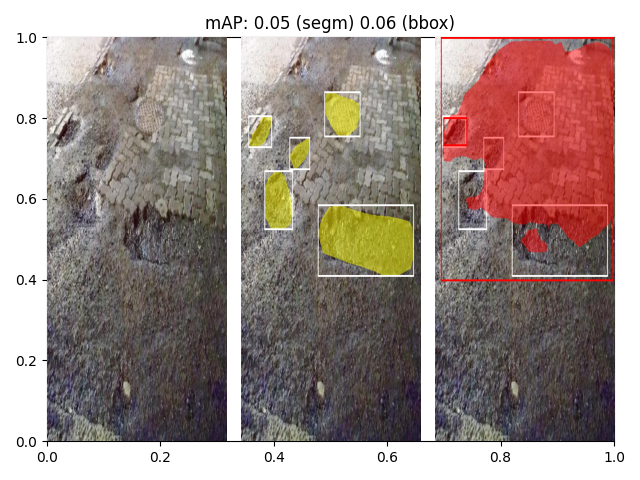
\includegraphics[width=1\linewidth]{Images/qualitative/bad.png}
    \end{minipage}\hfill
    \begin{minipage}{0.5\textwidth}
        \centering
        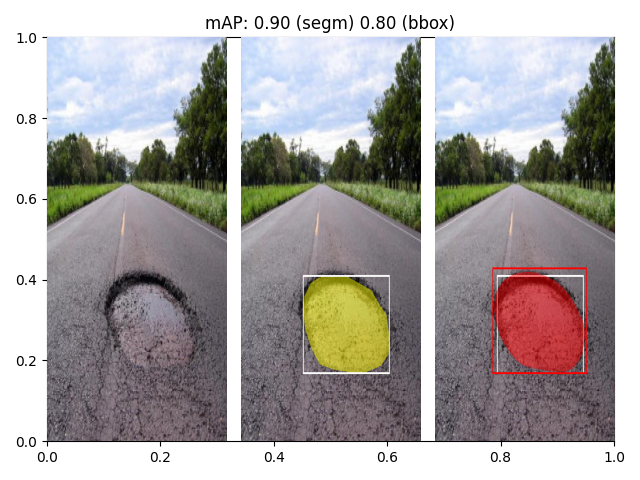
\includegraphics[width=1\linewidth]{Images/qualitative/easy.png}
    \end{minipage}
    \caption{On the right an easy example with a good prediction. On the left a bad prediction even if the problem wasn't a difficult one.}
    \label{fig:good_bad_predictions}

    \vspace{1cm}
    \begin{minipage}{0.50\textwidth}
        \centering
        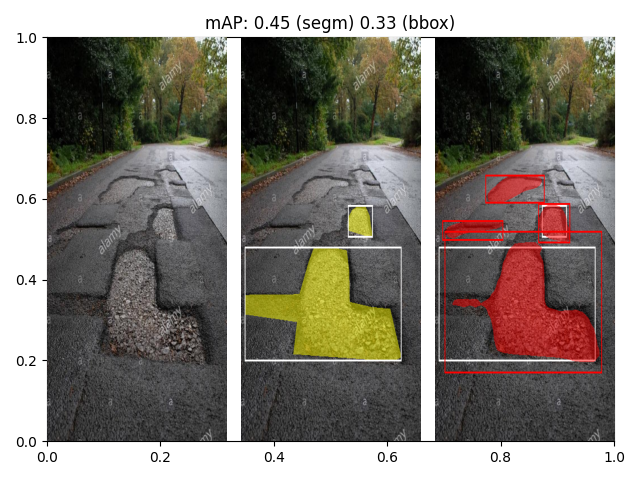
\includegraphics[width=1\linewidth]{Images/qualitative/bad_label.png}
    \end{minipage}\hfill
    \begin{minipage}{0.50\textwidth}
        \centering
        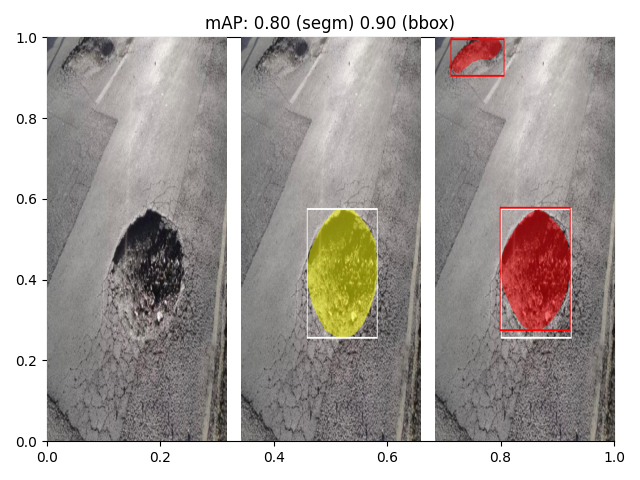
\includegraphics[width=1\linewidth]{Images/qualitative/bad_label_4.png}
    \end{minipage}\hfill
    \vspace{0.5cm}
    \begin{minipage}{0.50\textwidth}
        \centering
        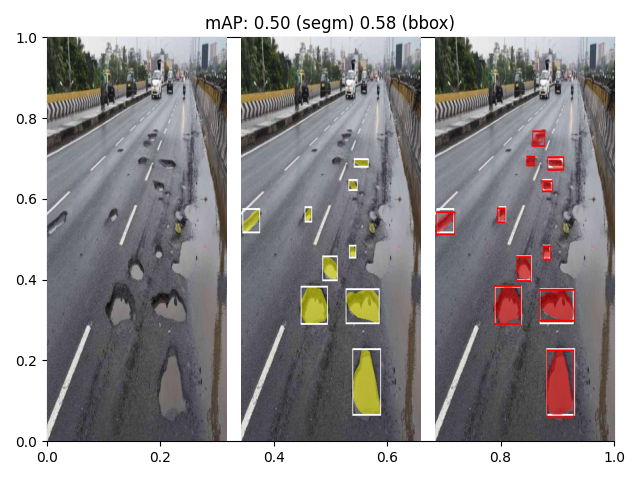
\includegraphics[width=1\linewidth]{Images/qualitative/bad_label_3.png}
    \end{minipage}\hfill
    \begin{minipage}{0.50\textwidth}
        \centering
        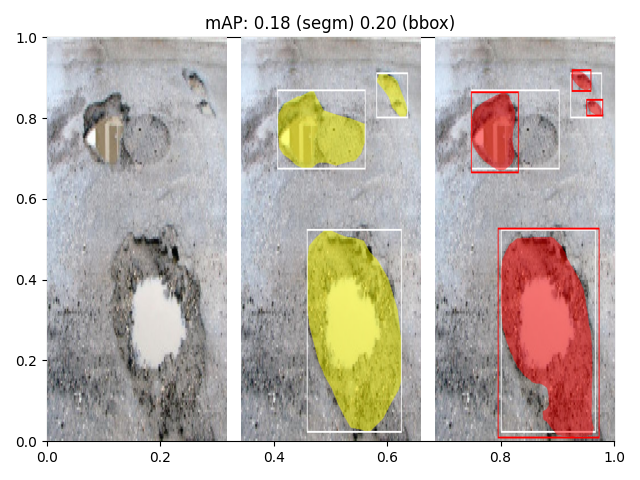
\includegraphics[width=1\linewidth]{Images/qualitative/bad_label_2.png}
    \end{minipage}\hfill

    \caption{Example of evident bad labelling.}
    \label{fig:bad_labelling}
\end{figure}


\begin{figure}[ht]
    \centering
    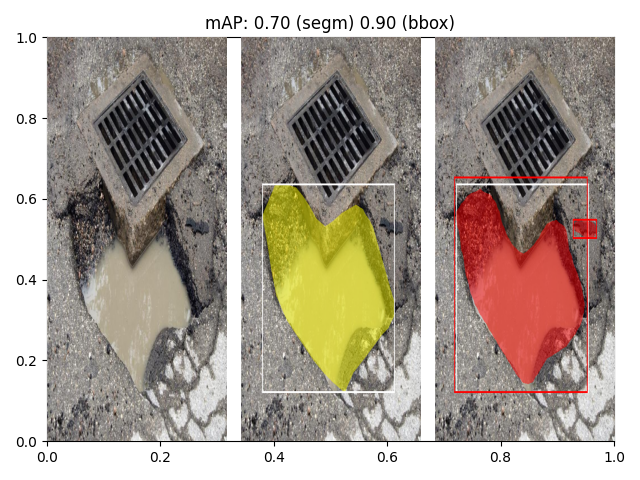
\includegraphics[width=0.8\textwidth]{Images/qualitative/manhole.png}
    \caption{Example of a manhole in the image. The model is able to ignore it and focus on the pothole}
    \label{fig:manhole}

    \vspace{1cm}

    \centering
    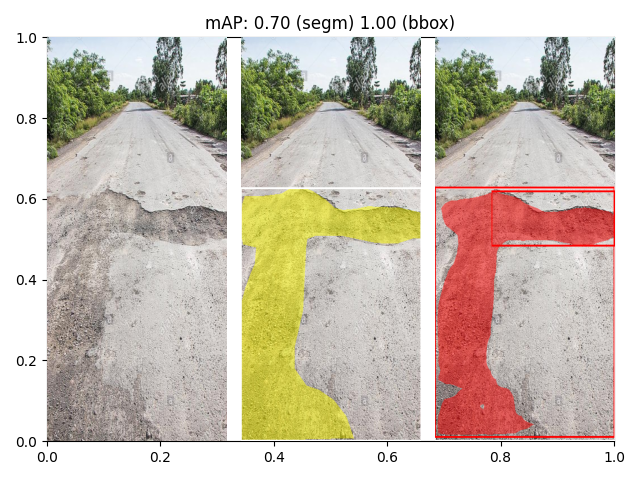
\includegraphics[width=0.8\textwidth]{Images/qualitative/nms.png}
    \caption{Example of multiple overlapping bounding box in the same pothole. The ambiguity is due to the diversity in depth of the pothole: the model knows the concept of depth and tries to predict the pothole in different depth levels.}
    \label{fig:nms}
\end{figure}

